\section{引言}
% 大背景(跳过)
% 相关方法的做法,这里应该强调的是guide,还有就是句子级的语义融合
% 图片中往往包含了更完整更丰富的语义信息,因此为了得到更准确的翻译,在翻译过程中加入图片信息成为了一种可行的方案。为了将图片信息融合到翻译中,广大研究者付出了很多的努力。早期的相关研究尝试在句子的编码过程中输入图片使编码结果更接近真实的语义,例如将图片特征作为基于RNN的翻译模型的初始化向量【】,亦或是将图片作为一个单词输入到模型中。也有一些方法以图片特征作为语义的中枢点,尝试为来自不同语言的文字或不同模态的语义信息创造一个统一的语义空间【】。同时,也有方法尝试在解码阶段输入图片,从而引入更多可参考的信息使解码的结果更准确。例如文献【】采用了注意力机制,在基于RNN或是基于Transformer的方法中均有着相似的应用。也有方法尝试
图片中往往包含着相比于文本描述更丰富的语义信息,因此为了得到更准确的翻译,在翻译过程中加入图片信息成为了一种可行的方案。为了将图片信息融合到翻译中,广大研究者付出了很多的努力。早期的相关研究尝试在句子的编码过程中输入图片使编码结果更接近真实的语义,例如将图片特征作为基于循环神经网络的翻译模型的初始化向量\pcite{elliott2015multilanguage,calixto2017incorporating},亦或是作为一个单词输入到模型中。也有一些方法以图片特征作为语义的中枢点,尝试为来自不同语言的文字或不同模态的语义信息创造一个统一的语义空间\pcite{kiros2014unifying,nakayama2017zero}。同时,也有方法尝试在解码阶段输入图片,从而引入更多可参考的信息使解码的结果更准确\pcite{calixto2017doubly,libovicky2018input}。这些方法普遍以句子为语义单位融合图片信息,这样做能够更充分地利用图片所包含的语义,也能最大化的辅助翻译过程。

%存在问题
然而,无论是通过简单地将图片输入翻译模型或是对模型结构进行复杂的设计,图片信息都很难为翻译带来理想的效果。一方面,输入图片信息不能够保证为翻译带来性能的提升;另一方面,当为待翻译句子提供与其内容不一致的图片时,对实际的翻译结果影响很小。这些问题说明一般的神经机器翻译模型对输入图片所提供的视觉信息并不敏感。

%本文做法
\begin{figure}[!htbp]
    \centering
    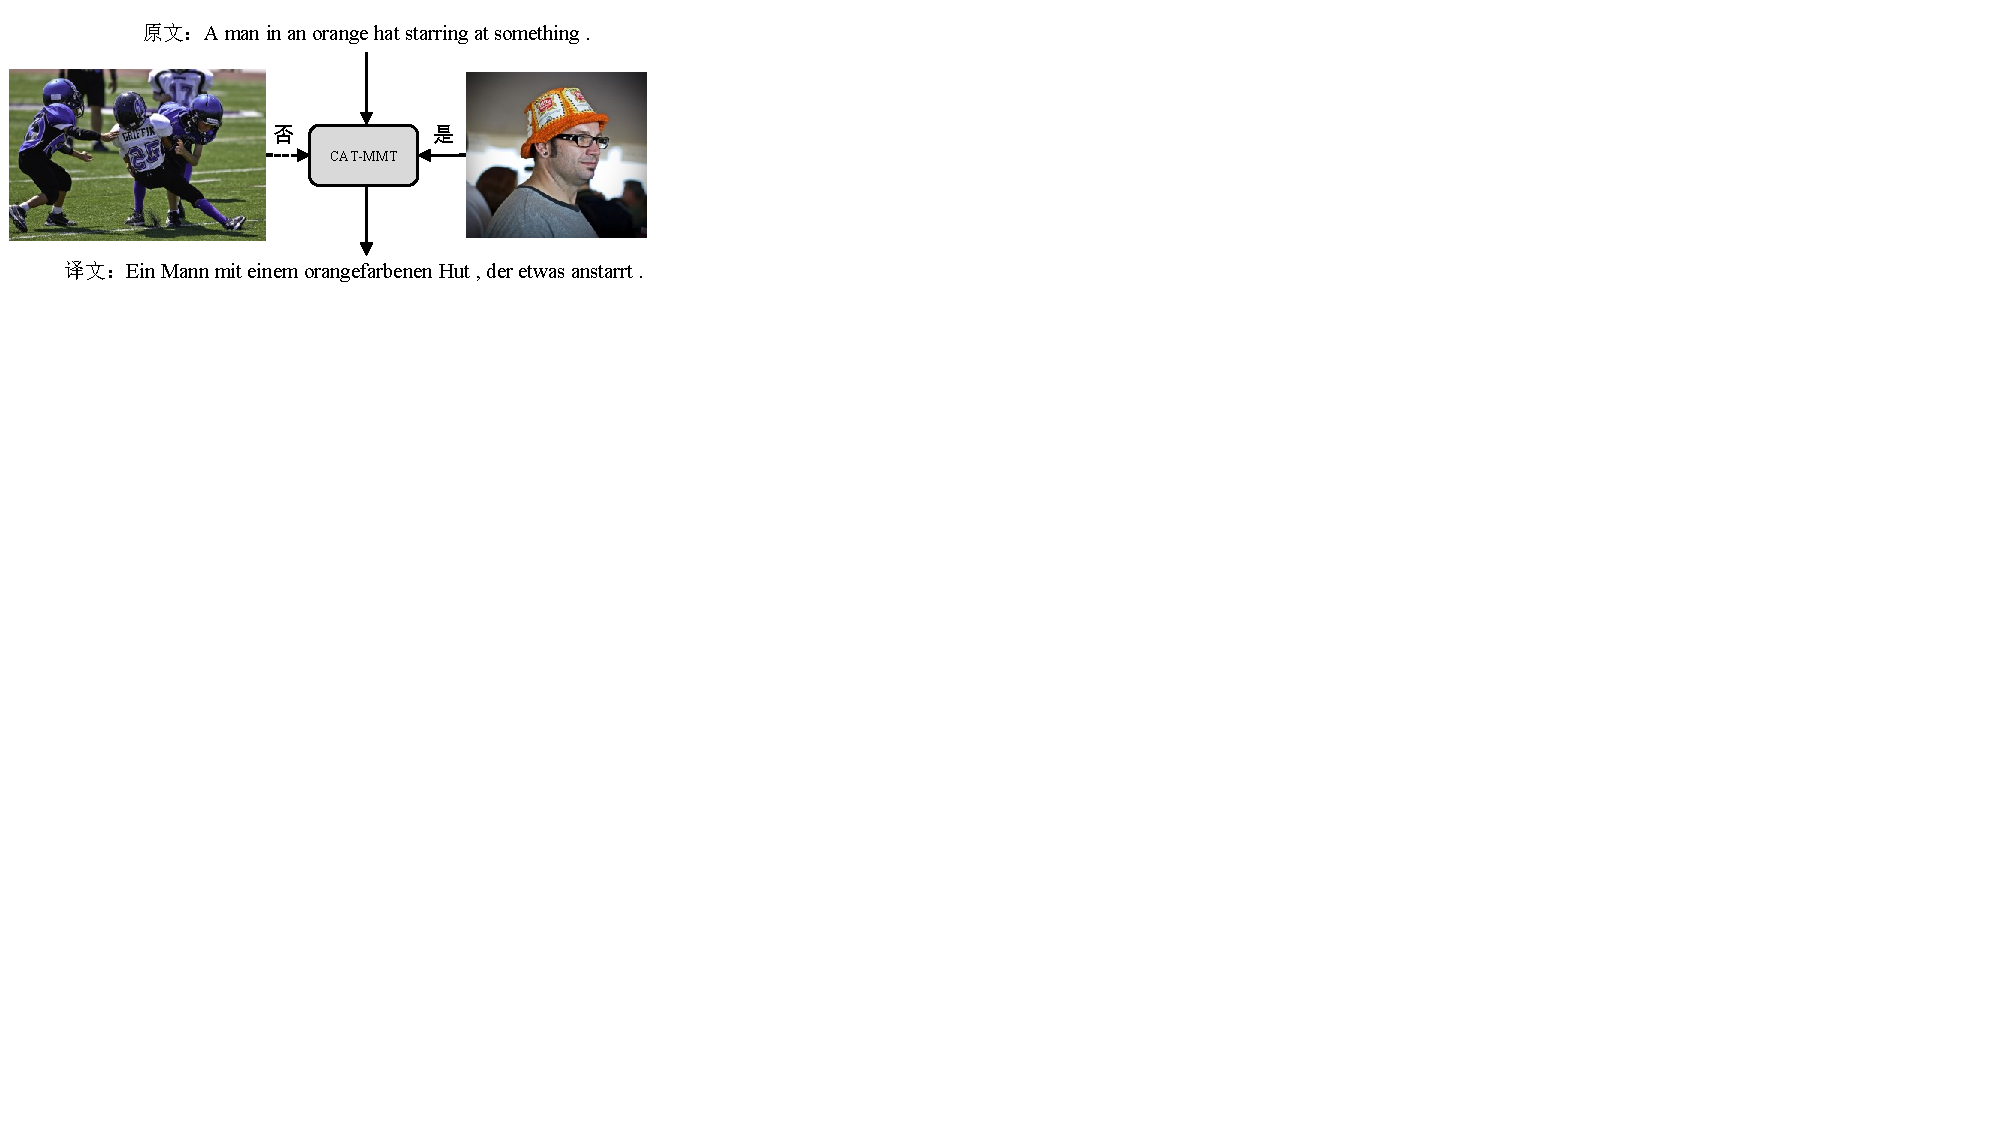
\includegraphics{Img/fig_5_example.pdf}
    \bicaption{引入对抗样本的神经机器翻译模型}{NMT model with adversarial samples}
    \label{fig:5_example}
\end{figure}
已有的相关工作表明在神经机器翻译任务中实现句子级的跨模态语义信息融合是很困难的。只有少部分的待翻译句子需要额外的输入图片作为信息的补充。大部分的翻译数据已经具备良好的双语对齐关系,这使得融合图片信息的端到端模型在面对更容易学习的并且是文本主导的翻译任务时,并不会过多地关注跨模态的信息对齐与融合。因此,针对神经机器翻译中的句子级跨模态语义融合方法,在讨论图片信息是否以及在哪些方面能够为翻译带来质量提升之前,应该更多地关注如何使模型具备从两个模态共同获得信息的能力。为此,本章提出了一种对比对抗训练(contrastive adversarial training, CAT)方法用于解决这个问题。首先,本章的模型输入与一般融合图片信息的翻译模型相似,为一个源语言句子和一张对应的图片。其中该图片中的视觉目标被提取出来,并一同输入到模型中。然后采用对比学习的方法拉近输入与译文在统一语义表示空间的距离。其中,译文作为锚点(anchor),将源语言句子与对应图片组合而成的图文输入作为正样本。为了使模型关注到图片所携带的视觉信息,本章将源语言句子与随机图片组合而成的图文输入作为负样本。如图\ref{fig:5_example}所示,应用该策略可以强迫翻译模型关注输入的源语言文本与输入图片的语义关系,从而实现句子级别的跨模态信息融合。

%具体贡献
本章主要贡献如下:

% 主要翻译性能上的贡献
(1)本章提出了一种基于图文对比对抗训练的神经机器翻译方法,又称CAT-NMT。在配合双向翻译训练后,对比对抗训练能够有效地为图片信息辅助式的神经机器翻译方法带来翻译准确率的提升。该方法在三个不同的翻译数据上得到了有效的提升。

% 主要动机上的贡献
(2)本章所提方法旨在将视觉信息融合到本文的表示中,
%试图通过图片信息加强翻译模型在编码过程中对源语言文本的表示能力,
试图利用图片信息辅助模型编码器完善对源语言文本的表示,
从而提升最终翻译的质量。在对抗实验的分析中可以观察到,CAT-NMT的翻译质量提升来源于成功地将图片信息融合到了文本表示中。因此,CAT方法达到了使神经机器翻译模型对视觉信息敏感的目的。

% 分析结果的贡献
(3)在对模型结果的分析中发现,为翻译输入随机图片或不输入图片时,带有歧义词较多的测试集受到的影响最大。该结果可以表明当神经机器翻译模型对视觉信息敏感时,对文本中存在歧义词问题的句子具有更好的翻译效果。